\documentclass[tikz,convert={density=300,outext=.png}]{standalone}
\usetikzlibrary{arrows.meta,graphs}
\usepackage{amsmath}
\begin{document}
    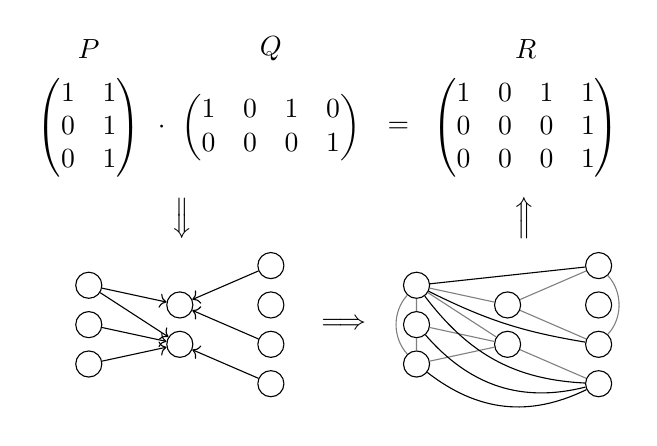
\begin{tikzpicture}[xscale=0.925]
  \tikzset{circ/.append style={circle, fill=black, inner sep = 0,
      minimum size = 0.15cm}} 
  \node (A) at (0,0) {$\begin{pmatrix} 1 & 1 \\ 0 & 1 \\ 0
          & 1 \end{pmatrix}$};
  \node (B) at (2.5,0) {$\begin{pmatrix} 1 & 0 & 1 & 0 \\ 0 & 0
        & 0 & 1 \end{pmatrix}$};
  \node (C) at (6,0) {$\begin{pmatrix} 1 & 0 & 1 & 1 \\
                    0 & 0 & 0 & 1 \\
                0 & 0 & 0 & 1\end{pmatrix}$};
  \node (cdot) at (1,0) {$\cdot$};
  \node (eq) at (4.25,0) {$=$};
  \node (lp) at (0,1) {$P$};
  \node (lq) at (2.5,1) {$Q$};
  \node (lr) at (6,1) {$R$};
  \node[rotate=270] at (1.25,-1.15) {$\Longrightarrow$};
  \node at (3.5,-2.5) {$\Longrightarrow$};
  \node[rotate=90] at (6,-1.15) {$\Longrightarrow$};
  \node[draw,circle] (a1) at (0,-2) {}; 
  \node[draw,circle] (a2) at (0,-2.5) {};
  \node[draw,circle] (a3) at (0,-3) {};
  \node[draw,circle] (b1) at (1.25,-2.25) {}; 
  \node[draw,circle] (b2) at (1.25,-2.75) {};
  \node[draw,circle] (c1) at (2.5,-1.75) {}; 
  \node[draw,circle] (c2) at (2.5,-2.25) {};
  \node[draw,circle] (c3) at (2.5,-2.75) {};
  \node[draw,circle] (c4) at (2.5,-3.25) {};
      \graph[use existing nodes] {
        a1 -> b1;
        a1 -> b2;
        a2 -> b2;
        a3 -> b2;
        c1 -> b1;
        c3 -> b1;
        c4 -> b2;
      };
  \node[draw,circle] (a1) at (0+4.5,-2) {}; 
  \node[draw,circle] (a2) at (0+4.5,-2.5) {};
  \node[draw,circle] (a3) at (0+4.5,-3) {};
  \node[draw,circle] (b1) at (1.25+4.5,-2.25) {}; 
  \node[draw,circle] (b2) at (1.25+4.5,-2.75) {};
  \node[draw,circle] (c1) at (2.5+4.5,-1.75) {}; 
  \node[draw,circle] (c2) at (2.5+4.5,-2.25) {};
  \node[draw,circle] (c3) at (2.5+4.5,-2.75) {};
  \node[draw,circle] (c4) at (2.5+4.5,-3.25) {};
      \graph[use existing nodes] {
        a1 --[thin,gray] b1;
        a1 --[thin,gray] b2;
        a2 --[thin,gray] b2;
        a3 --[thin,gray] b2;
        c1 --[thin,gray] b1;
        c3 --[thin,gray] b1;
        c4 --[thin,gray] b2; 
        a1 --[thin,gray] a2;
        a1 --[thin,gray,bend right=45] a3;
        a2 --[thin,gray] a3;
        c1 -- [thin,gray,bend left=45] c3;
        a1 -- c1;
        a1 --[bend right=8] c3;
        a1 --[bend right=24] c4;
        a2 --[bend right] c4;
        a3 --[bend right] c4;
      };
  \end{tikzpicture}
\end{document}



